\icode{E-MI-MU-L3-261030-001}
（多选）
如图所示，固定在竖直平面内的光滑圆环的最高点有一个光滑的小孔，质量为\(m\)的小球套在圆环上，一根细线的下端系着小球，上端穿过小孔用手拉住。现拉动细线，使小球沿圆环缓慢上移，在移动过程中手对线的拉力\(F\)和环对小球的弹力\(F_N\)的大小变化情况是\paren[]

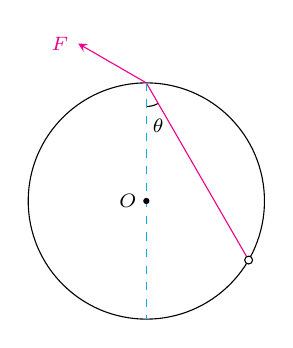
\begin{tikzpicture}[>=stealth,font=\scriptsize]
	\draw (0,0) circle(1.5) (0,1.2) arc(-90:-60:.3);
	\draw[->,magenta] (-30:1.5)--(0,1.5)--++(150:1)node[left]{\(F\)};
	\draw[fill=white] (-30:1.5) circle(0.05);
	\draw[dashed,cyan] (0,1.5)--(0,-1.5);
	\fill (0,0)node[left]{\(O\)} circle(.04);
	\node at(.15,.95){\(\theta\)};
\end{tikzpicture}
\begin{choices}
	\item\(F\)减小
	\item\(F\)不变
	\item\(F_N\)不变
	\item\(F_N\)增大
\end{choices}
\begin{answer}
	AC\quad 提示：对小环受力分析，构建力的三角形，找相似
\end{answer}